\documentclass[11pt, oneside]{article}  
\usepackage[margin=1in]{geometry}     
\geometry{letterpaper}                   	
\usepackage{graphicx}			
\usepackage{amssymb}
\usepackage{amsmath}
\usepackage[usenames,dvipsnames,svgnames,table]{xcolor}
\usepackage{multicol}
\usepackage{xypic}


\title{Things Linear\\
\Large (like algebra and models and stuff)}
\author{Schwartz} %
\setcounter{section}{-1}

\begin{document}
\maketitle

\section{Synopsis}
Glorified cheat sheet

\section{LinAlg}

\subsection{inner product -- \emph{dot product}}

${}$\\
\noindent $||x||_2, ||x||_1,$ and $||x||_\infty$% \sqrt{x^Tx} = \sqrt{dot(x,x)}, sum|x_i|, max_i|x_i|   


$$A_{n\times m} \cdot B_{m\times p} \quad = \quad C_{n\times p}$$

\hspace{1em}$\left[
\vcenter{\xymatrix{
\quad\ar[rr]^r &  & \quad \\
& \vdots &\\
\ar[rr] &  &  \\}}
\right] \cdot $
$\left[
\vcenter{\xymatrix{
\ar[dd]_c &  & \ar[dd] \\
& \cdots &\\
  &  &  \\}}
\right] 
$$\quad=\quad$$\left[
\vcenter{\xymatrix{
  \\
\;\; C_{r,c} = A_{r} \cdot B_{c} \;\; \\ %dot\left( \right)  
  \\}}
\right]$


\subsection{outer product (a.k.a. \emph{a whole lot of inner product}) } 

  
\hspace{8em} $\left[
\vcenter{\xymatrix{
\ar[dd]\\
\\
\\}}
\right]^A_{n\times 1}$
$\left[\vcenter{\xymatrix{
\ar[rr] &  &  \\}}
\right]^B_{1\times m} $
$\quad=\quad$
$\left[
\vcenter{\xymatrix{
 \\
\;\; C_{r,c} = A_{r} \times B_{c} \;\; \\
  \\}}
\right]_{n\times m} $ 
    
    
\subsection{broadcasting}
A little bit like outer product, but also \emph{a whole lot more}...

  
$\left[
\vcenter{\xymatrix{
\ar[dd]\\
\\
\\}}
\right]^A_{n\times 1}$
*\;\;\;\;
$\left[\vcenter{\xymatrix{
\ar[rr] &  &  \\}}
\right]^B_{1\times m} $
$\quad=\quad\;\;$
$\left[\vcenter{\xymatrix{
\ar[rr] &  &  \\}}
\right]^B_{1\times m} $
*\;\;\;
$\left[
\vcenter{\xymatrix{
\ar[dd]\\
\\
\\}}
\right]^A_{n\times 1}$
$=\quad\;$
$\left[
\vcenter{\xymatrix{
 \\
\;\; C_{r,c} = A_{r} \times B_{c} \;\; \\
  \\}}
\right]_{n\times m} $ \\${}$\\


\noindent \begin{minipage}{0.38\linewidth} 
\subsection{matrix things and such}
\begin{itemize}
\item MM is !\emph{communative} but is 
\item[] associative and distributive 
\item $(AB)^T = B^TA^T$
\item If $A = A^T$ then $A$ is  \emph{symmetric}
\item[] $\frac{1}{2}A + \frac{1}{2}A^T$ is symmetric
\item tr$ABC =$ tr$BCA=$ tr$CAB$ 
\item[] 
\item $\nabla_x a^Tx = a$, and if $A$ symmetric 
\item[] $\nabla_x x^TAx = 2Ax$ 
\item[] $\nabla_x^2 x^TAx = 2A$
\item[] 
\item[]
\item $(AB)^{-1} = B^{-1}A^{-1}$  
\item $(A^{-1})^T = (A^T)^{-1}$ 
\end{itemize}
 \vspace{-.8em}
\end{minipage}
\begin{minipage}{0.62\linewidth} 
\subsection{Spaces}
\begin{itemize}  
\item 
$\textrm{span}\{x_1,\cdots,x_m\} = \mathcal{R}\left(A=\left[x_1,\cdots,x_m\right] \right)$
\item[] $\textcolor{white}{\textrm{span}\{x_1,\cdots,x_m\}} = \left\{v \in \mathbb{R}^n: v=\overset{m}{\underset{i=1}{\sum}} \alpha_i x_i \right\}$ 
\item[] \textcolor{white}{$\textrm{span}\{x_1,\cdots,x_n\} =$ } 
with $x_i\in \mathbb{R}^n$ and $\alpha_i \in \mathbb{R} $
\item[] \underline{Relevant for LM's:}
\item[] $\quad$ The \emph{projection} of $y$ onto $\mathcal{R}(A = {[}x_1,\cdots,x_m{]})$ is \\
$$\underset{v \in \textrm{span}\{x_1,\cdots,x_m\}}{\textrm{argmin}} ||y - v||_2 = A(A^TA)^{-1}A^Ty$$
\item[] \underline{Relevant for SVM's:}
\item[] $\quad$ The \emph{projection} of $y$ onto $a$ is $\frac{a^T}{||a||}y = \frac{a^T}{\sqrt{a^Ta}}y$
\item[]
\item The \emph{nullspace} of $A \in \mathbb{R}^{n\times m}$ $\mathcal{N}(A) = \left\{x \in \mathbb{R}^m: Ax=\textbf{0} \right\}$ 
\item[] Why are $\mathcal{R}(A^T)$ and $\mathcal{N}(A)$ \emph{orthogonal complements}?
\item[] I.e.,  $\{w: w=u+v, u \in \mathcal{R}(A^T), v \in \mathcal{N}(A)\} = \mathbb{R}^m$ 
\item[] and $\mathcal{R}(A^T) \cap \mathcal{N}(A) = \{\textbf{0}\}$
\end{itemize}  
\end{minipage}



\subsection{Invertability}
\begin{minipage}{0.5\linewidth} 
\begin{itemize}
\item column rank is row rank is rank
\item rank($A_{(n,m)}$) $\leq$ min($m,n$), \emph{full} if equal
\item $A^{-1}A = I$ if $A \in \mathbb{R}^{n\times n}$ is \emph{full rank} 
\item[] otherwise A is \emph{singular/non-invertable}
\item $(A^{-1})^T = (A^T)^{-1}$
\item $U^TU = I \;(= UU^T)$ for \emph{orthonormal} $U$ % $||Ux||_2=||x||_2$
\item[]
\item $|det \;A| = \textrm{abs}(|A|)$ is the volume of the $\mathbb{R}^n$-parallelotope   
 formed by the vectors of $A$ 
\item $|A| = 0$ if $A$ is not full rank
\item[] I.e., $A$ singular (non-invertable)
\item $|A^{-1}|=|A|^{-1}$, $|A| = |A^T|$, $|AB| = |A||B|$
\end{itemize}  
\end{minipage}
\begin{minipage}{0.5\linewidth} 
\begin{itemize}  

% doesn't *have* to be symmetric. And also same story for negative (semi)definite here... just showed +
\item  $A=A^T$ is \emph{positive semidefinite} if $x^TAx \geq 0$
\item[]  and \emph{positive definite} if $x^TAx > 0$     
\item[] $\Longrightarrow$ full rank (i.e., \emph{non-singular/nvertable}) 
\item For full rank $A_{(n,m)}$ with $n>m$
\item[] the \emph{Gram matrix} $A^TA$ is positive definite
\item[] \underline{Relevant for LM's:}
\item[] $\quad$ $X^TX$ is inverted in the least squares fit $$X(X^TX)^{-1}X^Ty$$
\item[]
\item $A^{-1} = \frac{1}{|A|}\textrm{adj}(A) \in \mathbb{R}^{n\times n}$
\item[] $\textrm{adj}(A)_{i,j}=(-1)^{i+j}|A_{-i,-j}|$ 
\end{itemize}  
\end{minipage}

\subsection{Eigens}

\begin{itemize}
\item An \emph{eigenvector} $\left(x \not = \textbf{0} \textrm{ in } \mathbb{C}^n\right)$ and
\emph{eigenvalue} $(\lambda)$ pair of $A \in \mathbb{R}^{n\times n}$ satisfy 
$$Ax = \lambda x$$ 
\item Solutions for $(\lambda I - A) x = 0$ exist if $(\lambda I - A)$ is singular/the nullspace $\mathcal{N}(\lambda I - A) \not = \{\textbf{0}\}$  
\item[]\hspace{15.5em}[so that rank$\left((\lambda I - A)^T\right)= $ rank$\left(\lambda I - A\right)$ is not full] \\
\item In which case eigenvalue solutions to $|\lambda I - A| = 0$ can be used to solve for eigenvectors in 
$$(\lambda I - A) x = 0$$
\item And for eigenvalues $\lambda_1,\cdots \lambda_n$ of $A$ we have that  
$$ \textrm{tr}A = \sum_{i=1}^n \lambda_i \quad \textrm{ and } \quad |A| = \prod_{i=1}^n \lambda_i
\quad \textrm{ and } \quad \textrm{rank}(A) = \sum_{i=1}^n 1_{{[}\lambda_i\not=0{]}}$$

\item \textcolor{gray}{Quiz: what are the eigens for (i) diagonal matrix $D$ and (ii) non-singular $A$?}
% diagonal values and those normalized columns -- i.e., the orthonormal columns
% A^{-1} Ax =  A^{-1} \lambda x 
% 0 =  (A^{-1} \lambda - I)x: null space
\item For $A = A^T$ we have that (i) $\lambda_1,\cdots \lambda_n \in \mathbb{R}^n$  and (ii)
the eigenvectors are \emph{orthonormal} 
\item[] \underline{Relevant for MVN:} \\
All the eigenvalues of $\Sigma$ must be non zero so that $\Sigma^{-1}$ exists 
\item For linearly independent eigenvectors $X = {[}x_1,\cdots x_n{]}$ and 
associated eigenvalues $\Lambda = \textrm{diag}(\lambda_1,\cdots \lambda_n)$ 
$$AX = X\Lambda \textrm{ implies that } A = X\Lambda X^{-1} \textrm{ is \emph{diagonalizable}}$$ 
\item[] \underline{Relevant for PCA:} \\
Diagonalization a.k.a. \emph{spectral} or \emph{eigenvalue} decomposition 
is a special case of the \emph{singular value decomposition} which uses the covariance/correlation matrix rather than the data matrix 

%There are several decompositions with various applications in data analysis, e.g., 
%the, \emph{Cholesky} decomposition provides efficiency , LU decompositions) 
 

\item{} \textcolor{gray}{Quiz: $A^{-1}$ for diagonalizable $A$?
What sign are the eigenvalues of positive definite $A$?}
%A^{-1}  = (U\Lambda U^T)^{-1} = (\Lambda U^T)^{-1}U^{-1} = U \Lambda^{-1}U^T   

%$$A = U\Lambda U^T \quad \textrm{ and } \quad z^TAz = z^TU\Lambda U^Tz = y^T\Lambda y = \sum_{i=1}^{n} \lambda_iy_i^2 $$
%\item[] $\quad \quad$ so that $A$ is \emph{positive} definite if $\lambda_i > 0$ for all $i$ 
%or \emph{negative} definite if $\lambda_i < 0$ for all $i$ 

\end{itemize}



\section{Regression}

The range of the (full rank) $n$ samples $p$ predictors covariate (or design) matrix $\mathcal{R}(X)$
is the space (of dimension $p < n$) of all possible predictions of $y \in \mathbb{R}^n$
$$\mathcal{Y} = X\boldsymbol{\beta}, \textrm{ for } \boldsymbol{\beta} \in \mathbb{R}^p$$

\noindent The projection of $y$ onto $\mathcal{R}(X)$ is $\hat y$ is 
\begin{align*} % requires amsmath; align* for no eq. number
\underset{X\boldsymbol{\beta}}{\textrm{min}} \; || X\boldsymbol{\beta} - y ||_2 = {}& 
\underset{X\boldsymbol{\beta}}{\textrm{min}} \;  \left(\left(X\boldsymbol{\beta} - y\right)^T \left(X\boldsymbol{\beta} - y\right) \right) \\
= {}& 
\underset{X\boldsymbol{\beta}}{\textrm{min}} \; \left( \boldsymbol{\beta}^TX^TX\boldsymbol{\beta} - 2X^Ty\boldsymbol{\beta} + y^Ty \right) 
\end{align*}

\noindent which (by taking the derivative) is maximized at 
$$\boldsymbol{\beta} = \left(X^TX\right)^{-1}X^Ty$$
%\newpage

\subsection{Linear Models}


\noindent \begin{minipage}{0.4\linewidth} 
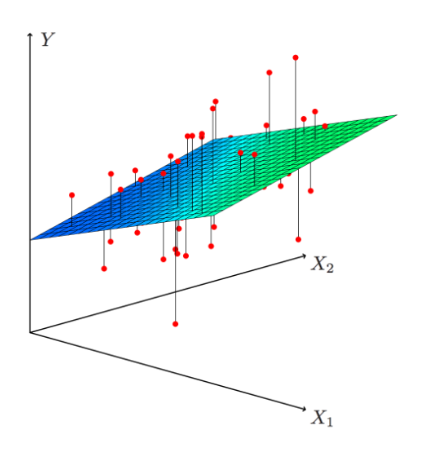
\includegraphics[width=2.25in]{OLS2.png} 
\end{minipage}
\begin{minipage}{0.55\linewidth} 
\vspace{-2em}
\begin{align*}
y_i ={}& \beta_0+\beta_1X_{i1} + \cdots + \beta_pX_{ip} + \epsilon_i,  \;  \epsilon_i \sim \textrm{N}(0,\sigma^2) \\ 
\hat y_i ={}& \beta_0+\beta_1X_{i1} + \cdots + \beta_pX_{ip} \\
\end{align*}

\begin{itemize}
\item Assumptions  -- when do they matter? 
% normality, homoskedasticity, independence, linear form, fixed X
% stats people care about diagnostics -- do you?
\item Higher order terms -- what does ``linear'' mean? 
\item Challenges interpreting coefficients? 
\item The role of rank($X$) and multicollinearity? % centering/scaling
\item Significance testing and model building?
% forward/backwards selection, AIC/BIC/Mallow's C_p
\end{itemize}

\end{minipage}

   
\subsection{Fit}

\begin{table}[h!]
\centering
\begin{tabular}{|c|c|c|c|}
\hline
Total Variation & Total Error & Average Error & Proportion Modeled\\
&&&\\
&&$RSE = \sqrt{\frac{1}{n-p-1}RSS}$ & $R^2 = \frac{TSS - RSS}{TSS}$ \\
$TSS = \sum_{i=1}^n(y_i - \bar y)^2$ &  $RSS = \sum_{i=1}^n(y_i - \hat y_i)^2$ & &\\
&&$\textcolor{white}{RSE^2} = \sqrt{\frac{\sum_{i=1}^n(y_i - \hat y_i)^2}{n-p-1}}$ &$\textcolor{white}{R} = 1-\frac{RSS}{TSS}$\\
&&&\\ \hline
\end{tabular}
\end{table}

\vspace{-1em}
\begin{figure}[h!]
\centering
\fbox{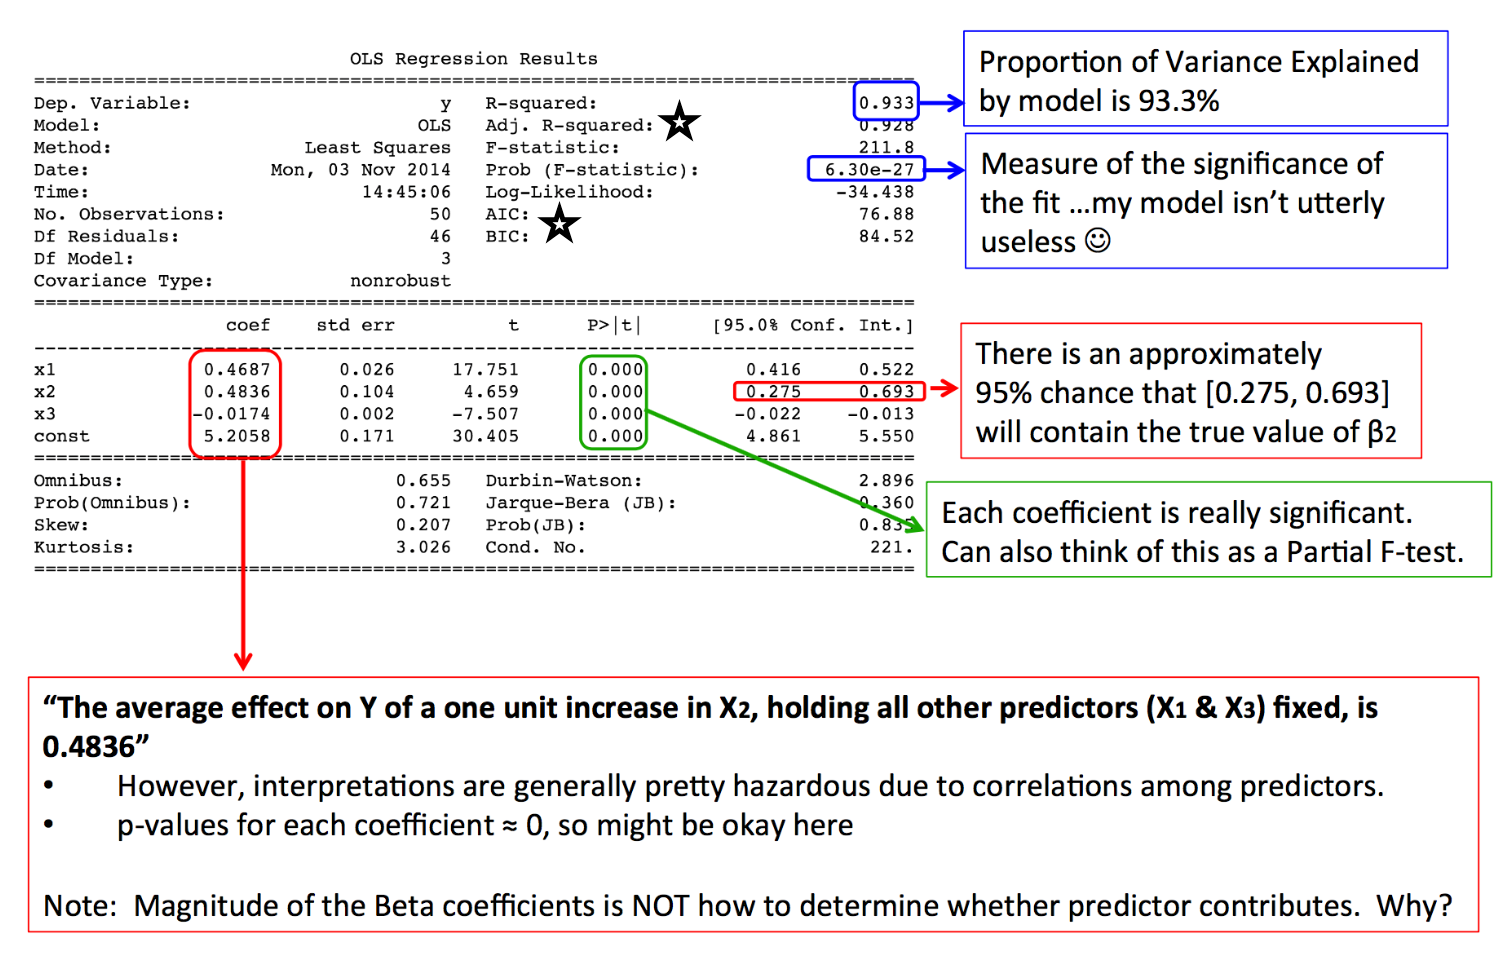
\includegraphics[width=6.4in]{OLS.png}}
\end{figure}

\section{Overfitting}

\vspace{-.5em}

\noindent \begin{minipage}{0.55\linewidth} 
Let $y_0 = \theta + \epsilon_0$ with $\theta = f(x_0)$ and $\epsilon \sim \textrm{N}(0,\sigma^2_\epsilon)$\\

For estimator $\hat \theta = \hat f(x_0),$

\begin{align*}
MSE ={}&  \frac{1}{n}\sum_i \left(y_i - \hat \theta \right)^2 \approx 
\textrm{E}\left[\left(y_i - \hat \theta \right)^2\right] \\
={}&
\sigma^2_{\hat \theta} + \left(\textrm{E}{[}\hat \theta{]}-\theta\right)^2 + \sigma^2_\epsilon \\ 
={}& \textcolor{gray}{\textrm{Variance $+$ Bias$^2$ $+$ Noise}} \\ \\
MSE(\hat \theta) ={}& \textrm{E}\left[\left(\hat \theta - \theta\right)^2\right] \\
={}&
\sigma^2_{\hat \theta} + \left(\textrm{E}{[}\hat \theta{]}-\theta\right)^2 \\
={}& \textcolor{gray}{\textrm{Variance $+$ Bias$^2$}}
% there is an easy proof of thish
\end{align*}
\end{minipage}
\begin{minipage}{0.5\linewidth} 

\vspace{1.75em}
\fbox{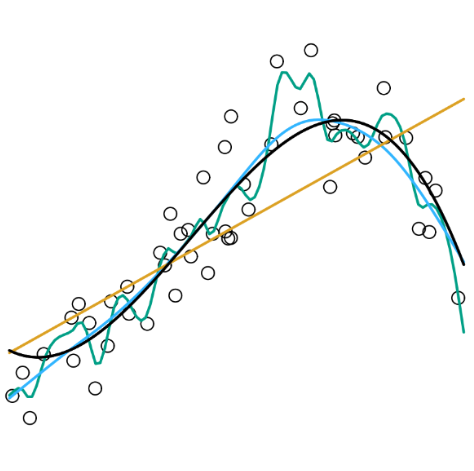
\includegraphics[width=2.9in]{varbiastradeoff.png}}\\

\hspace{4em}\textcolor{gray}{The variance/bias tradeoff}
\end{minipage}

\subsection{ $K$-folds cross-validation}

\vspace{-.5em}

\noindent \begin{minipage}{0.5\linewidth} 
\vspace{.4em}
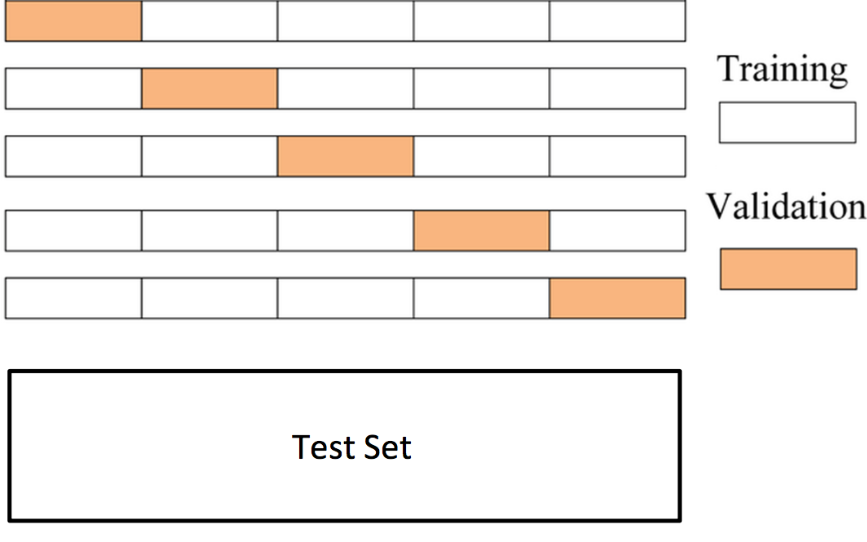
\includegraphics[width=3.2in]{kfold.png}\\
\vspace{.1em}

\end{minipage}
\begin{minipage}{0.5\linewidth} 
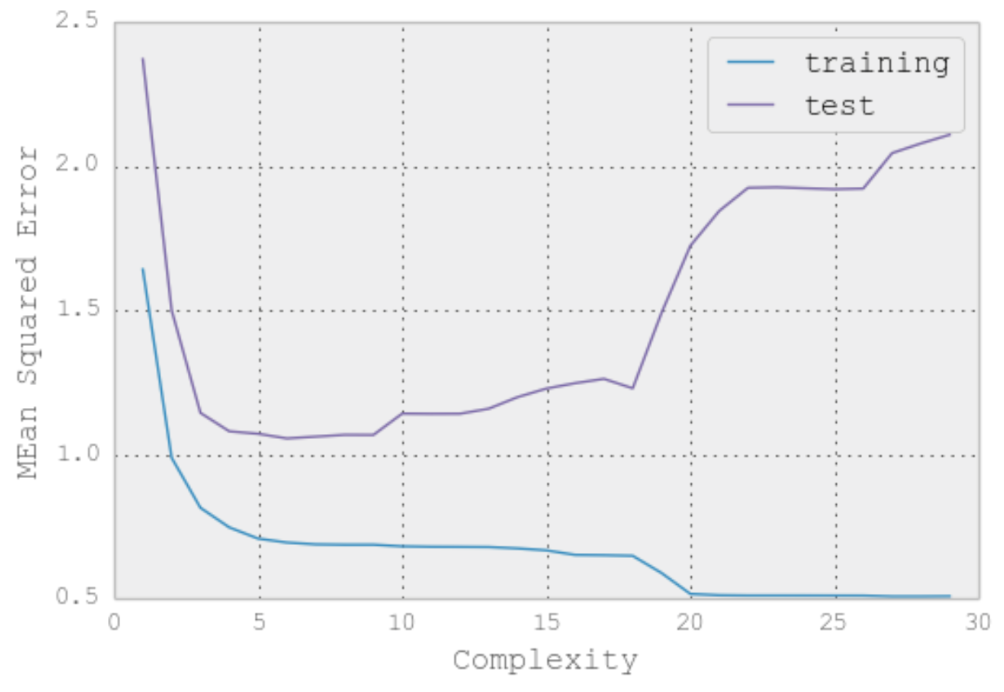
\includegraphics[width=3.35in]{kfolds2.png}
\end{minipage}


\subsection{Regularization}

\begin{minipage}{0.555\linewidth} 
\begin{align*}
\textrm{LS} ={}& \displaystyle \underset{\boldsymbol{\beta}}{\textrm{min}} \; || X\boldsymbol{\beta} - y ||_2 \quad\quad\quad\quad\quad\;\;\; \textcolor{gray}{(\textrm{no penalty})} \\
\textrm{Ridge} ={}& \displaystyle \underset{\boldsymbol{\beta}}{\textrm{min}} \; || X\boldsymbol{\beta} - y ||_2  + \lambda ||\beta||_2  \quad\quad \textcolor{gray}{(L_2 \textrm{penalty})}\\
\textrm{Lasso} ={}& \displaystyle \underset{\boldsymbol{\beta}}{\textrm{min}} \; || X\boldsymbol{\beta} - y ||_2  + \lambda ||\beta||_1 
\quad\quad \textcolor{gray}{(L_1 \textrm{penalty})} 
\end{align*}
Penalized coefficients \emph{not} scale equivariant!
\end{minipage}
\begin{minipage}{0.5\linewidth} 
\fbox{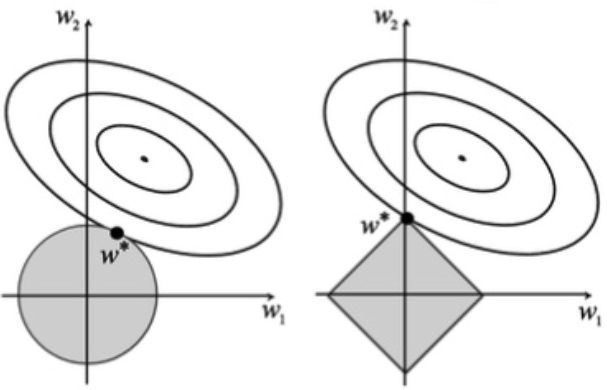
\includegraphics[width=2.8in]{L1L2.png}}
\end{minipage}

\newpage

\begin{figure}
\centering
 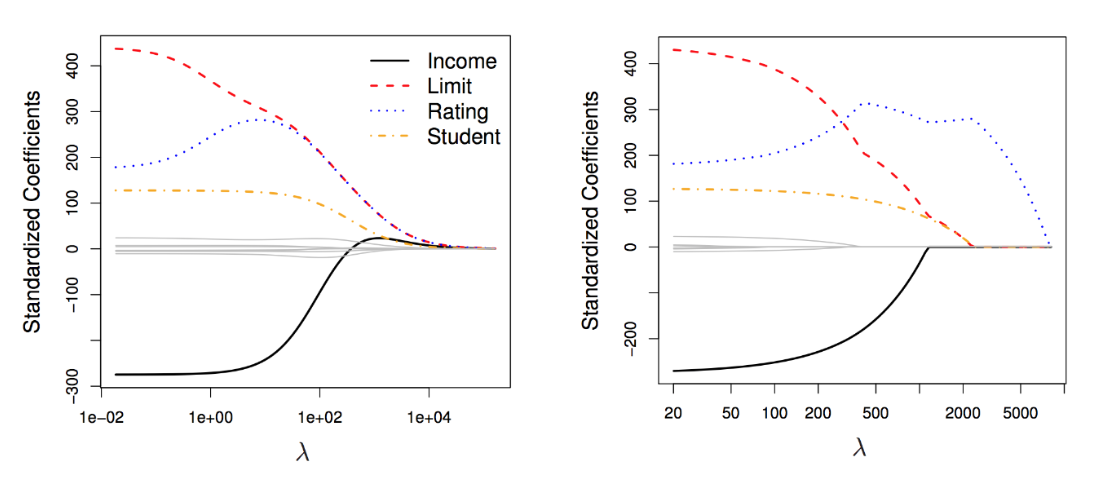
\includegraphics[width=5in]{regularize.png}

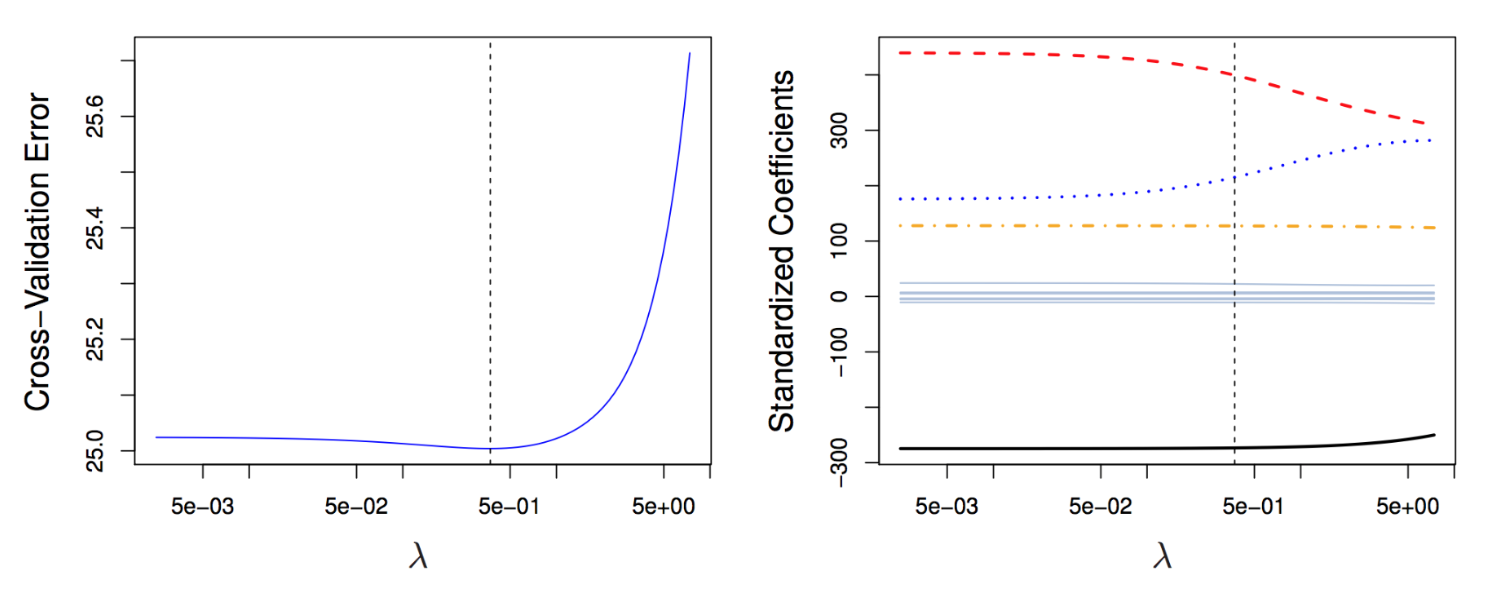
\includegraphics[width=5in]{chooseregularize.png}\\
\noindent Ridge (top left), Lasso (top right), and  cross-validation tuning parameter selection  (bottom row)
\end{figure}


\subsection{Summary}
\begin{tabular}{lll}
1. Model selection &2. Regularization &3. Dimension reduction (e.g., \emph{principal components reduction})
\end{tabular}

\subsection{Bonus: Bayesian regularization priors}

\begin{tabular}{rrrr}
\multicolumn{1}{c}{$\quad$Gausian} & \multicolumn{1}{c}{$\quad$Laplace} & \multicolumn{1}{c}{$\quad$Cauchy} & \multicolumn{1}{c}{$\quad$Horseshoe} \\
 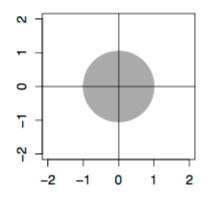
\includegraphics[width=1.55in]{regularization_prior3_R.png} &
 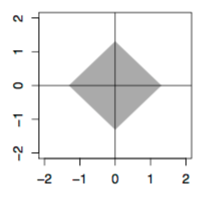
\includegraphics[width=1.5in]{regularization_prior3_L.png} &
  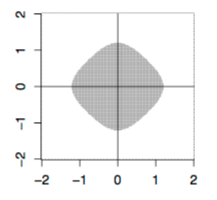
\includegraphics[width=1.55in]{regularization_prior3_C.png} &
 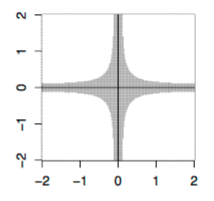
\includegraphics[width=1.5in]{regularization_prior3_H.png} \\
 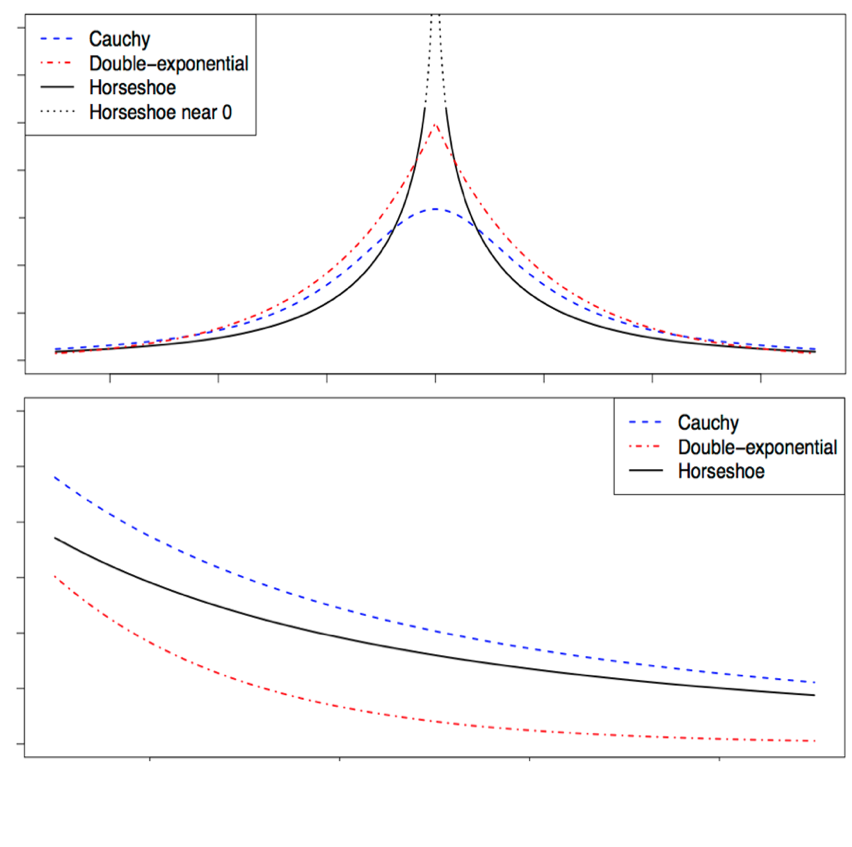
\includegraphics[width=1.15in]{regularization_prior2.png}\textcolor{white}{...}
 &
 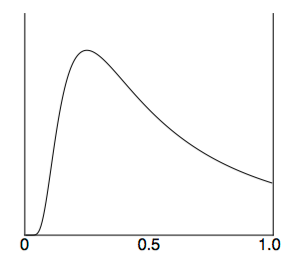
\includegraphics[width=1.3in]{regularization_prior4_L.png} &
  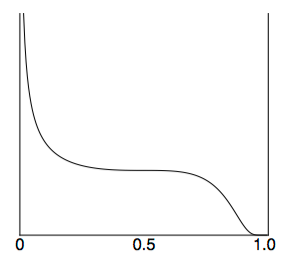
\includegraphics[width=1.3in]{regularization_prior4_C.png} &
 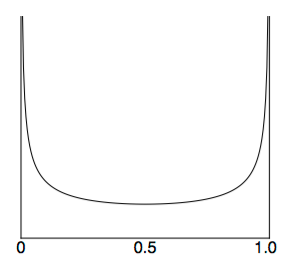
\includegraphics[width=1.3in]{regularization_prior4_H.png} \\
\multicolumn{1}{c}{$\quad$Tails}& \multicolumn{3}{c}{$\quad$Implied shrinkage prior profiles from none (0) to total (1) shrinkage}
  \end{tabular}
 



\newpage
\section{Logistic Regression}
% taxonomy of ML:
%Binary classification (can be extended to multinomial regression)
%Supervised Learning
%Linear -- it is a linear separator
%Technically: The log-odds is a linear function of the input
%fast & cheap
%Interpretable
%GLM
% regularization here?

\begin{itemize}
\item  The logit \emph{link function} $g(p) = \log\left(\frac{p}{1-p}\right)$ maps $p \in {[}0,1{]} \mapsto Z \in \mathbb{R}$
\item  For a binary outcome $Y$, setting E$\left[Y\right] = g^{-1}(Z) = \frac{\exp(Z)}{1+\exp(Z)}$ and $Z =  \beta_0 + \beta_1X_{1} + \cdots + \beta_mX_m$ 
$$Pr(Y=1|X)  = \frac{1}{1 + e^{-(\beta_0 + \beta_1X_{1} + \cdots + \beta_nX_m )}}$$
\item[] and 
$$ \exp(\beta_0)\exp(\beta_1X_{1})\cdots\exp(\beta_mX_{m}) = \frac{Pr(Y=1|X)}{Pr(Y=0|X)} $$ 
with  
$\exp(\beta_j)$  the multiplicative (logarithmic scale) \emph{odds} increase for a 1-unit increase in $X_{j}$
\end{itemize}

\noindent \begin{minipage}{0.55\linewidth} 

\begin{itemize}
\setlength\itemsep{0em}
\item True Positive ($TP$)
\item True Negative ($TN$)
\item False Positive ($FP$)\\ (Type I error)
\item False Negative ($FN$)\\ (Type II error, 1 - power)
\item[] 
\item Accuracy: $(TP+TN)/(TP+FP+FN+TN)$
\item F1 score: $2TP/(2TP+FP+FN)$
\item[] 
\item Sensitivity: $TP/(TP+FN)$\\ (power)
\item Specificity: $TN/(TN+FP)$\\ (1 - Type I error rate $\alpha$)
\item Positive Predictive Value: $TP/(TP+FP)$\\ (Precision)
\item Negative Predictive Value: $TN/(TN+FN)$\\ 
\item False Positive Rate: $FP/(FP+TN)$ \\(fall-out)
\item False \emph{Discovery} Rate: $FP/(FP+TP)$\\(1 - precision)
\item False \emph{Negative} Rate: $FN/(FN+TP)$\\(1 - sensitivity)
\end{itemize}
\end{minipage}
\begin{minipage}{0.5\linewidth} 
\hspace{1.2em}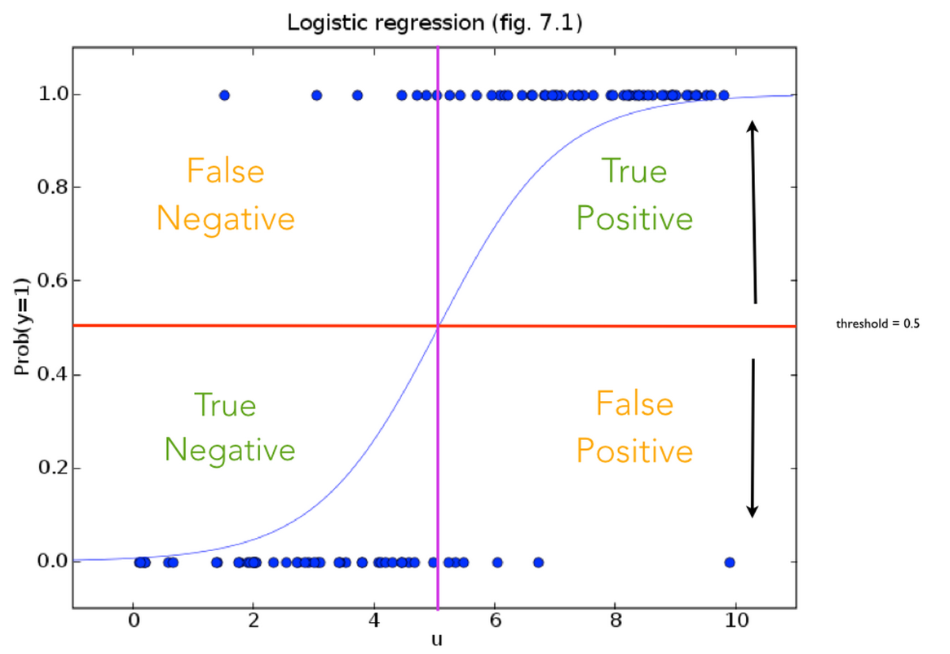
\includegraphics[width=3.5in]{logistic.png}

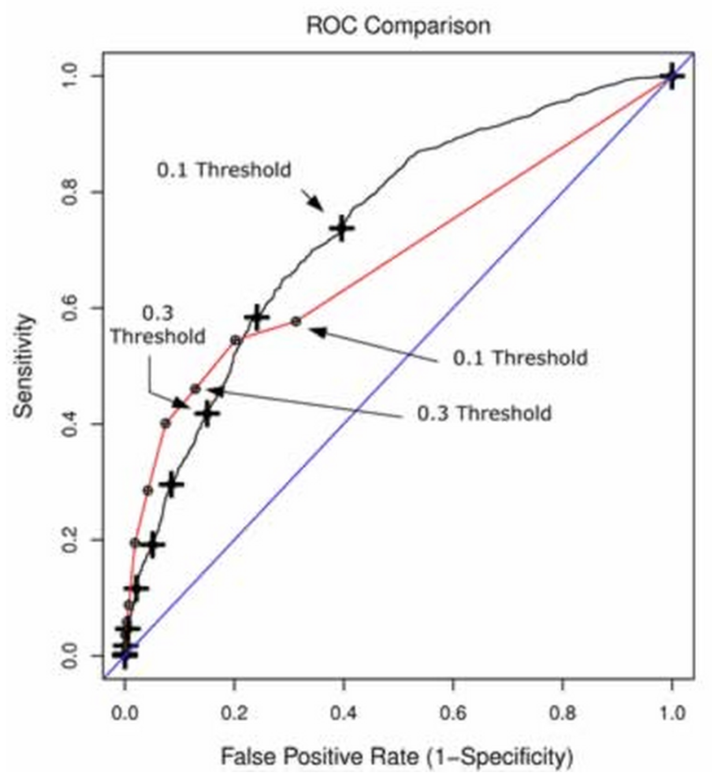
\includegraphics[width=3.175in]{roc.png}
\end{minipage}

\newpage


\section*{Appendix: classical model selection}
\fbox{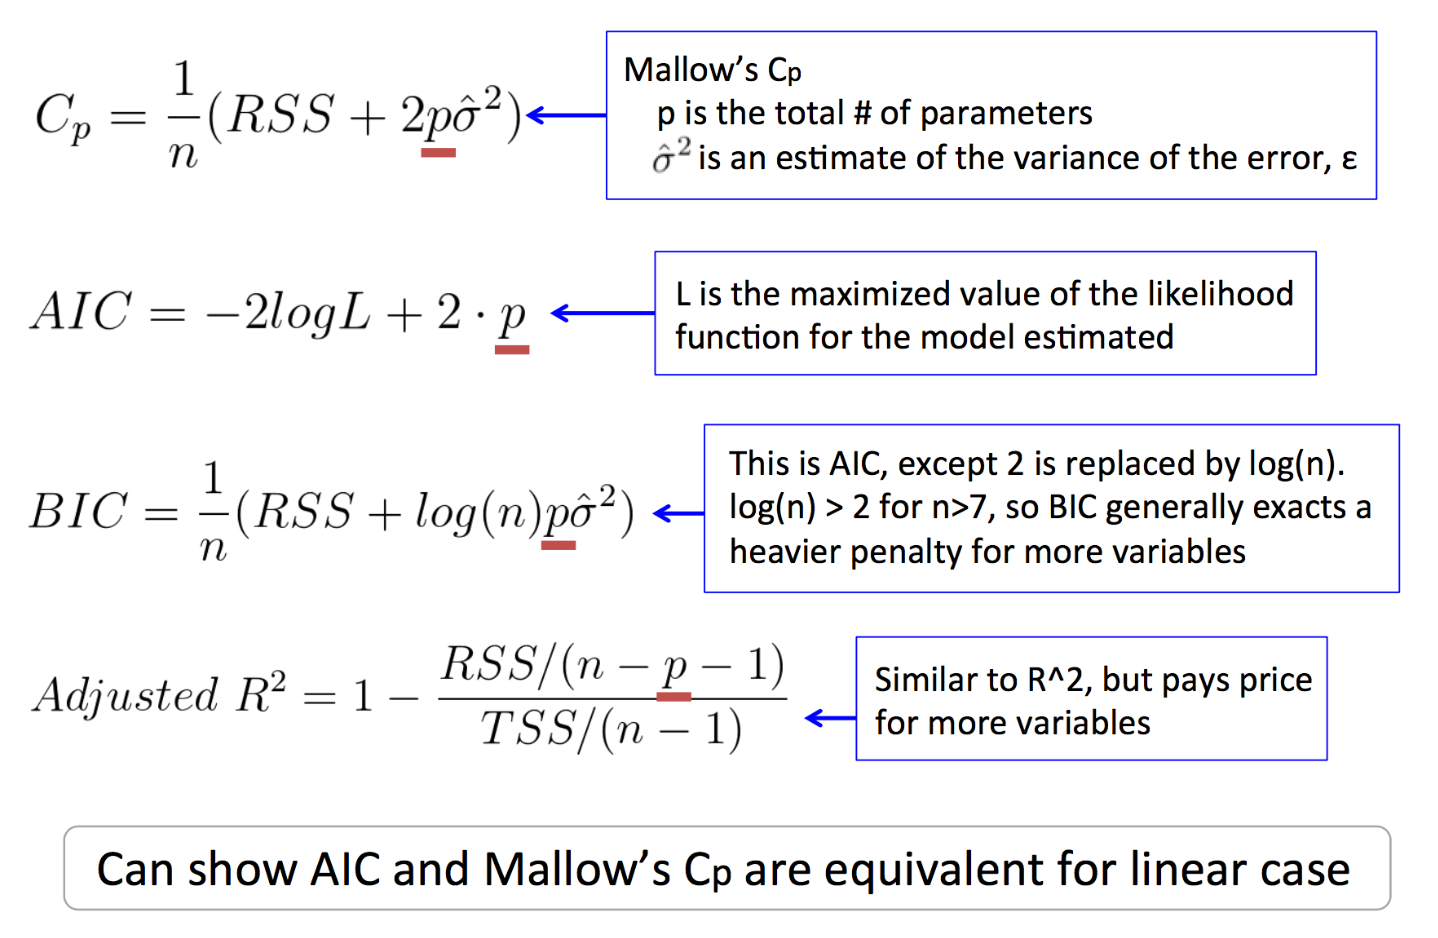
\includegraphics[width=6.5in]{model_comparision.png}}



\end{document}  
